
\documentclass[preprint,12pt]{elsarticle}

\usepackage[spanish]{babel}
\usepackage{amssymb}
\usepackage{graphicx}
\usepackage{lineno}
\usepackage[utf8]{inputenc}
\usepackage{url}
\usepackage{natbib} 
\usepackage{amsmath} 
\usepackage{amssymb} 

\begin{document}
	
	\begin{frontmatter} 

		\title{\huge MESA DE AYUDA}
		
		\author{Huichi Contreras, Franklin Carlos            (2016056193)}
		\author{Gonzales Cave, Angel Gabriel              	(2017057861)}
		\author{Condori Quispe, Yhónn Joel	         	(2016056358)} 
		\author{Pastor Mendoza, José Edilberto             	(2016055237)} 
		\address{Escuela Profesional de Ingeniería de Sistemas}
		\address{Universidad Privada de Tacna}
		\address{Tacna, Perú}
		
%% ABSTRACT --------------------------------------------------------------------------------------------------------------------

		\begin{abstract}
The proposal the design a help desk for the technical support area of the Tacna Private University arises due to the demand of user requests to solve basic problems in their computer equipment, the general objective of this project is to provide the necessary information for the user and in turn provide the basic knowledge to solve technical problems in the equipment.

		\end{abstract}

%% ----------------------------------------------------------------------------------------------------------------------------------

	\end{frontmatter}

%% RESUMEN ---------------------------------------------------------------------------------------------------------------------

\section{Resumen}
La propuesta de diseñar una mesa de ayuda para el área de soporte técnico de la Universidad Privada de Tacna surge debido a la demanda de solicitudes de los usuarios para resolver problemas básicos en sus equipos informáticos, el objetivo general de este proyecto es proporcionar la información necesaria para El usuario y a su vez proporcionan los conocimientos básicos para la resolución de problemas técnicos en el equipo.


%% ----------------------------------------------------------------------------------------------------------------------------------


%% INTRODUCION ----------------------------------------------------------------------------------------------------------------

\section{Introducción} 

EDITAR\\

%% ----------------------------------------------------------------------------------------------------------------------------------


%% TITULO  ------------------------------------------------------------------------------------------------------------

\section{Titulo}

EDITAR\\

%% ----------------------------------------------------------------------------------------------------------------------------------

%% AUTORES  ------------------------------------------------------------------------------------------------------------

\section{Autores}

EDITAR\\

%% ----------------------------------------------------------------------------------------------------------------------------------

%% PLANTEAMIENTO DEL PROBLEMA ------------------------------------------------------------------------------------------------------------

\section{Planteamiento del problema}

%%  SUBSECCION 

\subsection {\textbf{Problema}}

EDITAR\\

%%  SUBSECCION 

\subsection {\textbf{Justificacion}}

EDITAR\\

%%Ejemplo de cita
\cite{Gartner} 

\begin{itemize}
	\item x
	\item y
	\item z
\end{itemize}

%%  SUBSECCION 

\subsection {\textbf{Alcance}}

EDITAR\\

%% ----------------------------------------------------------------------------------------------------------------------------------

%% OBJETIVOS ------------------------------------------------------------------------------------------------------------

\section{Objetivos}

EDITAR\\

%% Ejemplo de inclusión de imagen
\begin{figure}[htb]
	\begin{center}
		% ESTA PARTE ME DA UN ERROR !!!
		%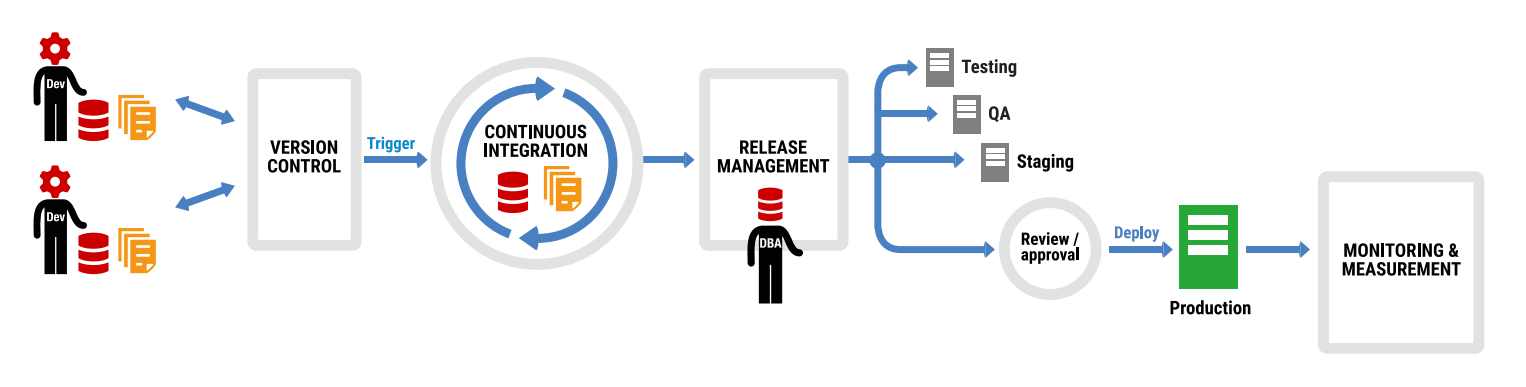
\includegraphics[width=14cm]{./IMAGENES/basededatos_1} 
		%\caption{Incluyendo la base de datos en DevOps}
	\end{center}
\end{figure}

%%  SUBSECCION 

\subsection{\textbf{General}}

EDITAR\\

\begin{itemize}

\item x
\item y
\item z

\end{itemize}

%%  SUBSECCION 

\subsection{\textbf{Especificos}}

EDITAR\\

%% ----------------------------------------------------------------------------------------------------------------------------------
 

%% REFERENTES TEORICOS ---------------------------------------------------------------------------------------------------

\section{Referentes Teoricos}

EDITAR\\

%% ----------------------------------------------------------------------------------------------------------------------------------


%% DESARROLLO DE LA PROPUESTA ---------------------------------------------------------------------------------------------------

\section{Desarrollo de la propuesta}

EDITAR\\

%%  SUBSECCION 

\subsection{\textbf{Tecnología de información}}

EDITAR\\

%%  SUBSECCION 

\subsection{\textbf{Metodología, técnicas usadas}}

EDITAR\\

%% ----------------------------------------------------------------------------------------------------------------------------------

%% CRONOGRAMA (PERSONAS, TIEMPO, OTROS RECURSOS) ---------------------------------------------------------------------------------------------------

\section{Cronograma}

EDITAR\\

%% ----------------------------------------------------------------------------------------------------------------------------------



%%  REFERENCIAS BIBLIOGRÁFICAS  (OJO NO TOCAR CON CITEP SOLO SE PONEN)------------------------------------------------------------------------------------------
	
	\newpage
	
	\bibliographystyle{apalike} 	%ESTILO
	\bibliography{BIBLIOGRAFIA}	 
	
	
\end{document}
